\documentclass[class=scrbook, crop=false]{standalone}
\usepackage[subpreambles=true]{standalone}
\ifstandalone
    % WARNING: Proceed with caution!

% -----------------------------------------------------------------------------------
% For package standalone
% -----------------------------------------------------------------------------------
\usepackage{import}

% -----------------------------------------------------------------------------------
% Language and typeset
% -----------------------------------------------------------------------------------
\usepackage[ngerman, english]{babel}

\usepackage{subcaption}
% Umlauts and other special characters (UTF-8)
% \usepackage[utf8]{inputenc}
\usepackage{fontspec}
\setsansfont{Arial}
% \usepackage[T1]{fontenc}  % Enable accented characters and umlauts
% LuaLatex doesn't need fontenc and uses UTF-8
% \usepackage{lmodern}  % Font face


% --------------------------------------------------------------------------------
% Page formatting
% --------------------------------------------------------------------------------
% Change the header/footer for chapter beginnings and normal pages
\usepackage[automark,headsepline]{scrlayer-scrpage}

% The package provides an easy and flexible user interface to customize the page
% layout, implementing auto-centering and auto-balancing mechanisms
% WARNING: WHEN CHANGING BCOR (Binding correction), the cover needs reworking!...
\newcommand{\theBCOR}{15mm}  % Define binding correction
\usepackage[
    bindingoffset=\theBCOR,
    % showframe, % Show boxes which indicate margins and paddings
    bottom = 3.5cm, % Margins
      left = 2.5cm,
     right = 2.5cm
] {geometry}

% The package 'float' provides a container for document objects which can not be
% broken over pages, such as tables and figures
% Needed for table and figure indexes  
\usepackage{float}

% support for landscape layout
\usepackage{lscape}

% support of \tablenotes command to add notes under table
\usepackage{threeparttable}

% To allow drawing more professional tables
\usepackage{booktabs}

% --------------------------------------------------------------------------------
% Contents
% --------------------------------------------------------------------------------
% Vector graphics (for Cover page)
\usepackage{tikz} 

% Allows additional parameters when including images
\usepackage{graphicx}

% Roman font family for all headings
\addtokomafont{disposition}{\rmfamily}

% Set the line spacing to 1.5
\usepackage[onehalfspacing]{setspace}

% Improves overall text spacing
% http://www.khirevich.com/latex/microtype/
\usepackage[stretch=10]{microtype}

% Math symbols like mu outside the math environment
\usepackage{textcomp}

% A comprehensive (SI) units package∗
% For defining SI units
\usepackage[
    range-units=single,         % Formatting ranges with single unit indication: 1 - 2 m
    range-phrase=-,             % Phrase for range: 1 - 2 m vs 1 to 2 m
    separate-uncertainty=true,  % sets +- between value and uncertainty 
    multi-part-units=repeat     % In expressions with multiple values (multi part numbers) 
                                % the unit is printed each time: 1 mm x 1 mm
] {siunitx}
% https://tex.stackexchange.com/questions/124488/multi-part-numbers-and-units-in-siunitx

% Allows Sourcecodes with highlighting 
\usepackage{listings}

% This package provides user control over the layout of the three basic list
% environments: enumerate, itemize and description
\usepackage{enumitem}
\setlist{nosep} % Remove the vertical space between \item elements in all lists

% ToDo Notes
% \setlength{\marginparwidth}{2cm}
\usepackage{todonotes}
\setuptodonotes{inline, inlinepar}
\reversemarginpar  % Put ToDo notes on the binding's side
% \usepackage{soul} % Colorful ToDo notes

% Check out colors here http://latexcolor.com/
\usepackage{xcolor}

\usepackage{amsmath}    % alignment of equations

% --------------------------------------------------------------------------------
% Other elements
% --------------------------------------------------------------------------------
% Blindtext: Organic looking text dummy
\usepackage{blindtext}

% Hyperlinks within the document (PDF)
% "hidelinks" hides visual highlighting of links
\usepackage[hidelinks]{hyperref}

% Package for Glossary and Index (Acronyms are listed in a separate list) 
\usepackage[acronym, nogroupskip]{glossaries}[=v4.49] % groupskip: alphabetic grouping of entries

\usepackage{xltabular}   % <------- FOR glossaries

% Integration and management of bibliographies
\usepackage{csquotes}   % backend=biber in biblatex needs this package
\usepackage[
    style=ieee,   % style of the bibliography, entries are sorted in alphabetic order. "ieee" is another common style.
    backend=biber,      % based on package 'biber' 
    bibencoding=ascii   % ASCII Text encoding; may use "utf8" instead
] {biblatex}

% --------------------------------------------------------------------------------
%                               PATHS & FILES
% --------------------------------------------------------------------------------
% Fix paths for standalone compiling
\ifstandalone
    \def \home {..}
\else
    \def \home {.}
\fi

% Package: scrlayer-scrpage
% \def \stylePath {\home/settings+/style/page}
\input{\home/settings+/style/page}  % Load page style

% Package: graphicx
\graphicspath{{\home/images/}}  % Set path to images

% Package: listings
\input{\home/settings+/style/code.tex}  % Set path to style file
\lstset{inputpath={\home/code/}} % Default path to code listings

% Package: glossaries
\input{\home/settings+/style/symbols}  % Set path to symbols list style file
\input{\home/settings+/style/acronyms}  % Set path to acronym list style file
% -------------------------------------------------------------------------------
%               Listing of all Glossary and Acronym Entries 
%                           use as shown below
% -------------------------------------------------------------------------------

% ==== EXEMPLARY ENTRY FOR SYMBOLS LIST =========================================

% ==== EXEMPLARY ENTRY FOR ACRONYMS LIST ========================================
% \newacronym{#label}{#acronym}{#long_form}

% define new command for custom arconym entry with only two arguments
% fabricates an easier way to use \newacronym 
\newcommand{\acroX}[2]{\newacronym{#1}{#1}{#2}}
% \acroX{label and arconym}{long name}
% \acroX{CD}               {Compact Disk}

\newcommand{\acroY}[3]{\newacronym{#1}{#2}{#3}}
% \arcoY{label}{acronym}{long name}
% \acroY{CD}   {cd}     {Compact Disk}
 
\newacronym{AEP}{AEP}{Imbalance price}
\newacronym{aFRR}{aFRR}{Automatic Frequency Restoration Reserve}


\newacronym{reBAP}{reBAP}{Uniform imbalance price}
\newacronym{TSO}{TSO}{Transmission System Operator}
\newacronym{FCR}{FCR}{Frequency Containment Reserve}
\newacronym{mFRR}{mFRR}{Manual Frequency Restoration Reserve}
\newacronym{BRP}{BRP}{Balancing Responsible Party}
\newacronym{SB}{SB}{System Balance}
\newacronym{VRE}{VRE}{variable renewable energy}
\newacronym{ID1}{ID1}{intraday index ID1}
\newacronym{MAE}{MAE}{mean average error}
\newacronym{RMSE}{RMSE}{root mean squared error}
\newacronym{MSE}{MSE}{mean squared error}
\newacronym{CRPS}{CRPS}{continuous ranked probabililty score}
\newacronym{GCC}{GCC}{Grid Control Cooperation}
\newacronym{IC}{IC}{Continuous intraday}
\newacronym{VWAP}{VWAP}{volume-weighted average price}
\newacronym{VID}{VID}{traded volume within the intraday market}
\newacronym{ID AEP}{ID AEP}{Intraday Average Energy Price}
\newacronym{FRR}{FRR}{Frequency Restoration Reserve}
\newacronym{TFT}{TFT}{Temporal Fusion Transformer}
\newacronym{DLM}{DLM}{Dynamic Linear Model}
\newacronym{GB}{GB}{Gradient Boosting}
\newacronym{RF}{RF}{Random Forest}
\newacronym{ARIMAX}{ARIMAX}{Autoregressive Integrated Moving Average with eXogenous variables}
\newacronym{xLSTM}{xLSTM}{Extended Long Short-Term Memory}
\newacronym{DWD}{DWD}{Deutscher Wetterdienst}
\newacronym{ENTSO-E}{ENTSO-E}{European Network of Transmission System Operators for Electricity}
\newacronym{IDA1}{IDA1}{Intraday auction 1}
\newacronym{MOSMIX}{MOSMIX}{Model Output Statistics-MIX}
\newacronym{mLSTM}{mLSTM}{memory-optimized LSTM}
\newacronym{sLSTM}{sLSTM}{speed-optimized LSTM}

% ==== EXEMPLARY ENTRY FOR MAIN GLOSSARY ========================================

    % \newglossaryentry{policy}{name={Policy},description={Im geschäftlichen Bereich bezeichnet Policy eine interne Leit- bzw. Richtlinie, die formal durch das Unternehmen dokumentiert und über ihr Management verantwortet wird}}
    % \newglossaryentry{pcie}{name={PCI Express},description={PCI Express („Peripheral Component Interconnect Express“, abgekürzt PCIe oder PCI-E) ist ein Standard zur Verbindung von Peripheriegeräten mit dem Chipsatz eines Hauptprozessors. PCIe ist der Nachfolger von PCI, PCI-X und AGP und bietet im Vergleich zu seinen Vorgängern eine höhere Datenübertragungsrate pro Pin.}}
    % \newglossaryentry{realnumber}
  % Load glossary, symbol and acronyms list

% Package: biblatex
\addbibresource{\home/references/references.bib}  % Set path to bib resources

% Custom variables
\input{\home/settings+/variables}
% --------------------------------------------------------------------------------
%                                   OPTIONAL
% --------------------------------------------------------------------------------


% Simple arithmetic for LaTeX commands
% \usepackage{calc}

% Document Elements
% -------------------

% Index
% \usepackage{imakeidx}

% compact Lists
%\usepackage{paralist}

% visual improvements for citations
% \usepackage{epigraph}

% Create pseudo code
% https://www.overleaf.com/learn/latex/Algorithms
% \usepackage{algorithm}
% \usepackage{algorithmic}
%\usepackage[noend]{algpseudocode}

% Formatting
% -------------------
% Tweaks for scrbook, redefines commands of other packages
% \usepackage{scrhack}

% Intelligent space separator (nice for superscript?)
% \usepackage{xspace}

% Allows breaks within tables
%\usepackage{tabularx}

% Allows for page breaks in tables
% \usepackage{longtable}

% allows modifying of captions
% \usepackage{caption}

% Multiline comments
%\usepackage{verbatim}

% % Custom colors
% \definecolor{dartmouthgreen}{rgb}{0.05, 0.5, 0.06}

% IF you want to define unicode characters
% \DeclareUnicodeCharacter{0229}{\c{e}}
% \DeclareUnicodeCharacter{0306}{\u{Z}}


% Document elements
% ------------------------------------

% Table package
% \usepackage{booktabs}

% Pie diagram
% \usepackage{datapie}

% Side by Side images
% \usepackage{subcaption}

% For landscape tables
%\usepackage{pdflscape}
%\usepackage{afterpage}

% Graphics can be flow around by text
%\usepackage{wrapfig}

\fi
\usepackage{subcaption}

% ----------------------------------------------------------------------------
%                               Discussion
% ----------------------------------------------------------------------------
\begin{document}

\chapter{Results and Discussion} % Overview text
\label{Chapter::Results and Discussion}
    In this chapter, the results of the thesis are presented and evaluated as well as, the approach of this thesis.

% Show your results and analyze them
% Explain why the results are the way they are and not different
% Go into possible measurement errors and why they occurred
% Look for anomalies and explain why they occur
\section{Results}
\label{Section::Results}

\subsection{Out of the box performance}
  
  \begin{table}[]
\centering
\begin{tabular}{l|l|l|l|l|l|l}
Model name &  RMSE & MAE & CRPS & 50\%-cov & 90\%-cov & 98\%-cov \\\hline
Naive intraday ID1 & 308.69 & 93.17 & 42.90 & 0.08 & 0.56 & 0.84 \\
Random forest & 241.37 & 90.22 & 52.38 & 0.32 & 0.80 & 0.94 \\
Arima & 358.75 & 100.5 & 42.04  & 0.21 & 0.61 & 0.81 \\
iTransformer & 367.50 & 111.66 & 42.40 & 0.09 & 0.66 & 0.84 \\
xLSTM &  156.40 & 107.65 & 51.41 & 0.25 & 0.68 & 0.84 \\
\end{tabular}
\caption{Out of the box performance for all models}
\label{Table::Out_of_the_box_performance}
\end{table}

\begin{figure}
  \centering
\begin{subfigure}{0.45\textwidth}
  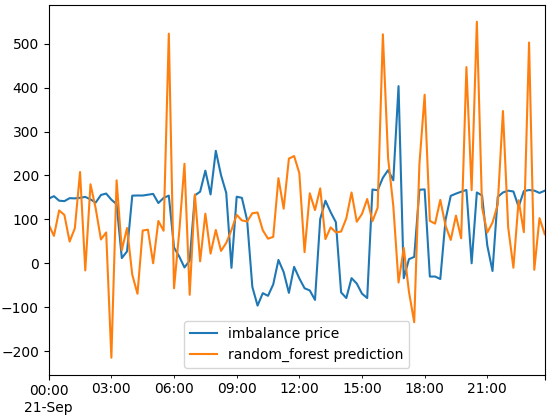
\includegraphics[width=\linewidth]{../images/results/random_forest_prediction.png}
  \caption{Predictions of random forest}
  \label{fig:sfig1}
\end{subfigure}
\begin{subfigure}{0.45\textwidth}
  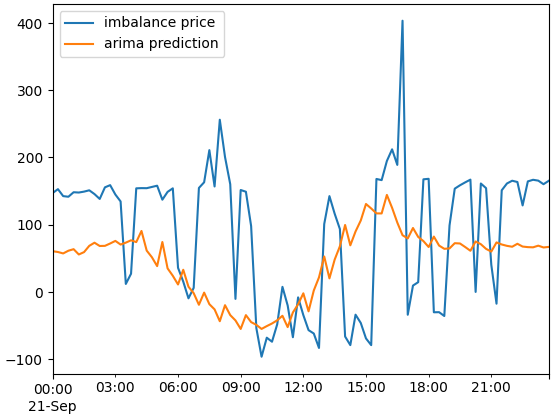
\includegraphics[width=\linewidth]{../images/results/arima_prediction.png}
  \caption{Predictions of ARIMA}
  \label{fig:sfig1}
\end{subfigure}
\begin{subfigure}{0.45\textwidth}
  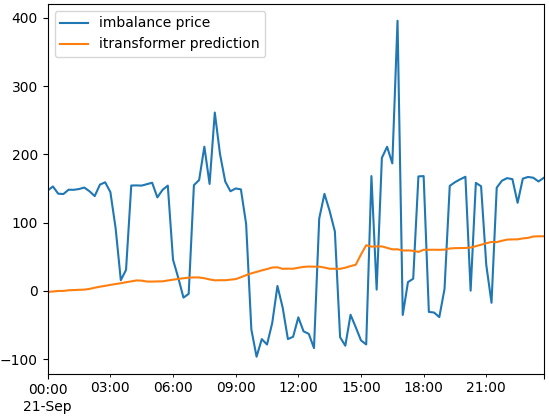
\includegraphics[width=\linewidth]{../images/results/itransformer_prediction.png}
  \caption{Predictions of iTransformer}
  \label{fig:sfig1}
\end{subfigure}
\begin{subfigure}{0.45\textwidth}
  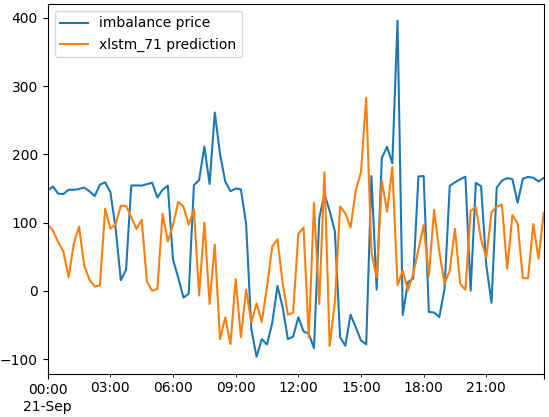
\includegraphics[width=\linewidth]{../images/results/xlstm_prediction.png}
  \caption{Predictions of xLSTM}
  \label{fig:sfig1}
\end{subfigure}
\caption{Predictions of the different models on example day}
\label{fig:fig}
\end{figure}

\subsection{Different xLSTM block structures}

  \begin{table}[]
\centering
\begin{tabular}{l|l|l|l|l|l|l}
Configuration name &  RMSE & MAE & CRPS & 50\%-cov & 90\%-cov & 98\%-cov \\\hline
xLSTM\_1\_0 & 154.87 & 109.50& 50.45& 0.30 & 0.76 & 0.87 \\
xLSTM\_0 \_1& 152.82 & 107.81 & 51.00 & 0.25 & 0.76 & 0.89 \\
xLSTM\_7\_1 & 156.40 & 107.65 & 51.41 & 0.25 & 0.68 & 0.84 \\
\end{tabular}
\caption{Performance for different xLSTM block configurations}
\label{Table::Performance_xLSTM}
\end{table}

\subsection{iTransformer variable sequence length}

 \begin{table}[]
\centering
\begin{tabular}{l|l|l|l|l|l|l}
 Configuration name &  RMSE & MAE & CRPS & 50\%-cov & 90\%-cov & 98\%-cov \\\hline
 iTransformer 96 seq & 367.50 & 111.66 & 42.40&0.09 & 0.66 & 0.84 \\
 iTransformer 192 seq & 368.45 &114.67& 43.07& 0.08 & 0.60	 & 0.83 \\
 iTransformer 384 seq & 362.46 & 107.08& 44.17	& 0.06	 &0.42	 & 0.84\\
\end{tabular}
\caption{iTransformer performance for different sequence lengths}
\label{Table::Performance_sequence_length}
\end{table}


\begin{figure}
  \centering
  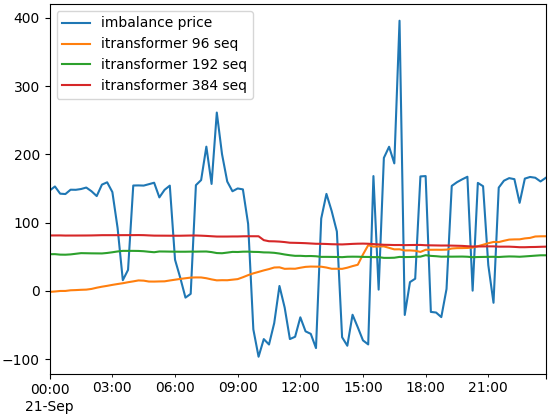
\includegraphics[width=.8\linewidth]{../images/results/itransformer_sequence_length_results.png}
  \caption{Predictions of iTransformers with different sequence lengths}
\label{Result::iTransformer_sequence_length}
\end{figure}

\subsection{iTransformer multiple target variables}

 \begin{table}[]
\centering
\begin{tabular}{l|l|l|l|l|l|l}
 Configuration name			&  RMSE 	& MAE 	& CRPS 	& 50\%-cov & 90\%-cov & 98\%-cov \\\hline
 iTransformer intraday indices 		& 367.32	&111.52	&42.40	&0.09			& 0.66	 & 0.84 \\
 iTransformer entsoe data		&  367.89	& 111.98 	&42.39	&0.09			& 0.66	 &0.83 \\
 iTransformer netzregelverbund 	& 367.55 	& 111.70	& 42.40	&0.09		 &0.66	 & 0.83\\
 iTransformer combined 		& 367.21 	& 111.42	& 42.40	& 0.10	 &0.66	 & 0.84\\
\end{tabular}
\caption{iTransformer performance for multiple target variables}
\label{Table::Performance_targets}
\end{table}


\begin{figure}
  \centering
\begin{subfigure}{0.45\textwidth}
  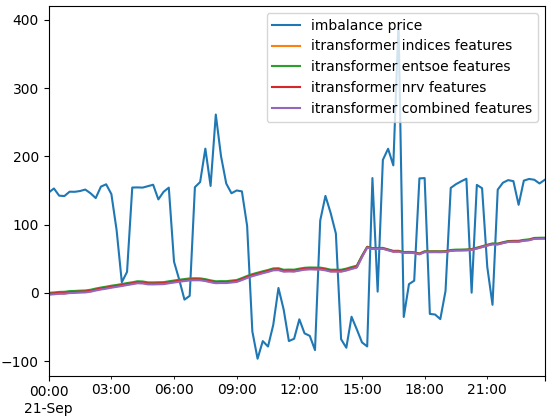
\includegraphics[width=\linewidth]{../images/results/itransformer_target_variables_aep.png}
  \caption{Predictions of models with imbalance price}
  \label{fig:sfig1}
\end{subfigure}
\begin{subfigure}{0.45\textwidth}
  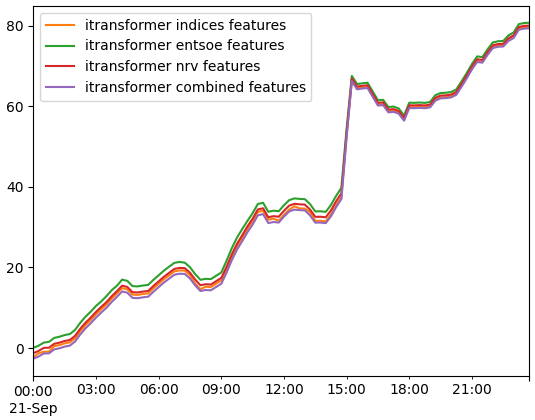
\includegraphics[width=\linewidth]{../images/results/itransformer_target_variables_alone.png}
  \caption{Predictions of models without imbalance price}
  \label{fig:sfig1}
\end{subfigure}
\caption{Predictions of iTransformers trained on multiple target variables}
\label{fig:fig}
\end{figure}


\subsection{iTransformer different prediction horizons}


 \begin{table}[]
\centering
\begin{tabular}{l|l|l|l|l|l|l}
 Configuration name			&  RMSE 	& MAE 	& CRPS 	& 50\%-cov & 90\%-cov & 98\%-cov \\\hline
 iTransformer 4 horizon			& 364.65	&108.98	&42.55	&0.12		& 0.64	 & 0.85 \\
 iTransformer 12 horizon			& 364.69	&108.93	&42.55	&0.12		& 0.63	 & 0.85 \\
 iTransformer 24 horizon			& 364.23	&108.26	&42.67	&0.13		& 0.60	 &0.85 \\
 iTransformer 48 horizon			& 367.78	&111.51	&42.39	&0.09		& 0.66	 & 0.84 \\
 iTransformer 96 horizon			& 368.28	&111.68	&42.45	&0.09		& 0.66	 & 0.84 \\
\end{tabular}
\caption{iTransformer performance for multiple target variables}
\label{Table::Performance_targets}
\end{table}

\begin{figure}
  \centering
\begin{subfigure}{0.45\textwidth}
  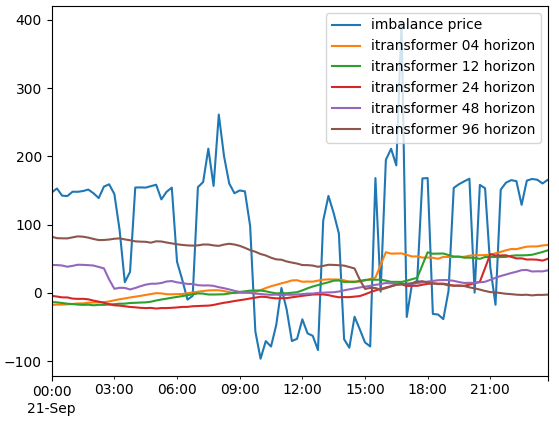
\includegraphics[width=\linewidth]{../images/results/itransformer_horizon_lengths.png}
  \caption{Predictions of models with imbalance price}
  \label{fig:sfig1}
\end{subfigure}
\begin{subfigure}{0.45\textwidth}
  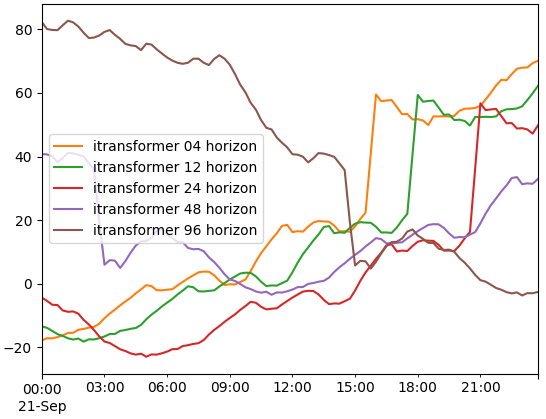
\includegraphics[width=\linewidth]{../images/results/itransformer_horizon_lengths_alone.png}
  \caption{Predictions of models without imbalance price}
  \label{fig:sfig1}
\end{subfigure}
\caption{Predictions of iTransformers trained on different forecasting horizons}
\label{fig:fig}
\end{figure}


\section{Analysis or Evaluation of Something}
\label{Section::Analysis or Evaluation of Something}    
    Text

\end{document}
